\documentclass{article}
\usepackage{amsmath}
\usepackage{amssymb}
\usepackage{graphicx}
\usepackage{hyperref}
\usepackage[version=4]{mhchem}


\begin{document}
Given \(\triangle A B C, A B=A C, B D \perp A C\). Prove: \(\angle C B D=\frac{1}{2} \angle A\).

Solution:
Method 1:\\
Draw \(C E \perp A B\). \(E\) is the foot of the perpendicular from \(C\) to \(A B\).\\
Points \(A, E, F\), and \(E\) are concyclic \(\left(\angle A E F+\angle A D F=90^{\circ}+\right.\)\\
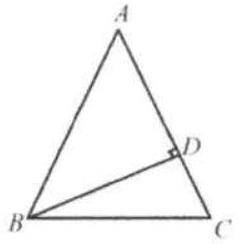
\includegraphics[width=\textwidth]{images/194(2).jpg} \(90^{\circ}=180^{\circ}\) ).\\
Connect \(A F\) and \(E D . \angle E A F=\angle D A F=\alpha\).\\
\(\angle E D F=\angle E A F=\alpha\). (both angles face the same arc \(E F\) ).

Note that \(E D / / B C\). Thus \(\angle E D B=\angle C B D=\alpha\).\\
That is, \(\angle C B D=\frac{1}{2} \angle A\).\\
\centering

\includegraphics[width=\textwidth]{images/194.jpg}

Method 2:\\
Draw \(A E \perp B C\). \(E\) is the foot of the perpendicular from \(A\) to \(B C\).\\
Points \(A, B, E\), and \(D\) are concyclic ( \(\angle A D B=\angle A E B=\) \(90^{\circ}\) ).\\
\(\angle D A E=\angle D B E=\alpha\) (both angles face the same arc \(D E\) ).\\
\centering
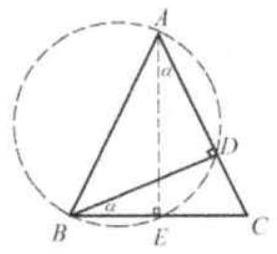
\includegraphics[width=\textwidth]{images/194(1).jpg}

Note that \(\triangle A B C\) is an isosceles triangle, \(A E\) is also the angle bisector of \(\angle A\).\\
Thus \(\angle C B D=\angle D B E=\alpha=\frac{1}{2} \angle A\).


\end{document}
